\documentclass[12pt, twoside]{article}
\usepackage[letterpaper, margin=1in, headsep=0.5in]{geometry}
\usepackage[english]{babel}
\usepackage[utf8]{inputenc}
\usepackage{amsmath}
\usepackage{amsfonts}
\usepackage{amssymb}
\usepackage{tikz}
\usetikzlibrary{quotes, angles}
\usepackage{graphicx}
\usepackage{enumitem}
\usepackage{multicol}
\usepackage{hyperref}

\newif\ifmeta
\metatrue %print standards and topics tags

\title{IB Mathematics}
\author{Chris Huson}
\date{March 2022}

\usepackage{fancyhdr}
\pagestyle{fancy}
\fancyhf{}
\renewcommand{\headrulewidth}{0pt} % disable the underline of the header
\raggedbottom

\fancyhead[LE]{\thepage}
\fancyhead[RO]{\thepage \\ Name: \hspace{4cm} \,\\}
\fancyhead[LO]{BECA / IB Math 5 Exponential functions \\* 4 March 2022}

\begin{document}
\subsubsection*{5.8 Classwork: Applications of exponential functions}
I can calculate continuous compounding \hfill CCSS.HSF.LE.A.2 \\[0.5cm]
$\displaystyle FV=PV \times \left(1+\frac{r}{100k} \right)^{kn}$
where FV is the future value,\\[0.25cm]
PV is the present value, n is the number of years, \\
 k is the number of compounding periods per year, \\
 r\% is the nominal annual rate of interest

\begin{enumerate}
\item Do Now: A six year investment of \$25,000 earns an annual interest rate of 6.125\%.
    \begin{enumerate}[itemsep=2cm]
    \item Find the future value at maturity (after 6 years) with annual compounding. 
    \item Find the value at maturity with monthly compounding.
    \end{enumerate} \vspace{2cm}

\item A rabbit population doubles every 4 weeks. There are currently five rabbits in a restricted area. With $t$ representing time, in weeks, then the population of rabbits can be modeled by \[\displaystyle P(t)=A \times b^{t/4}\]
%Alg2 Regents Jan2017
\begin{enumerate}[itemsep=0.75cm]
    \item Write down the value of $A$
    \item Write down the value of $b$
    \item About how many rabbits will there be in 98 days? \vspace{2cm}
    \item After how many weeks will there be approximately 160 rabbits?
\end{enumerate}

\newpage
\item Graph $y=300(0.89)^{2x}-10$ on the set of axes below.
    \begin{center}
        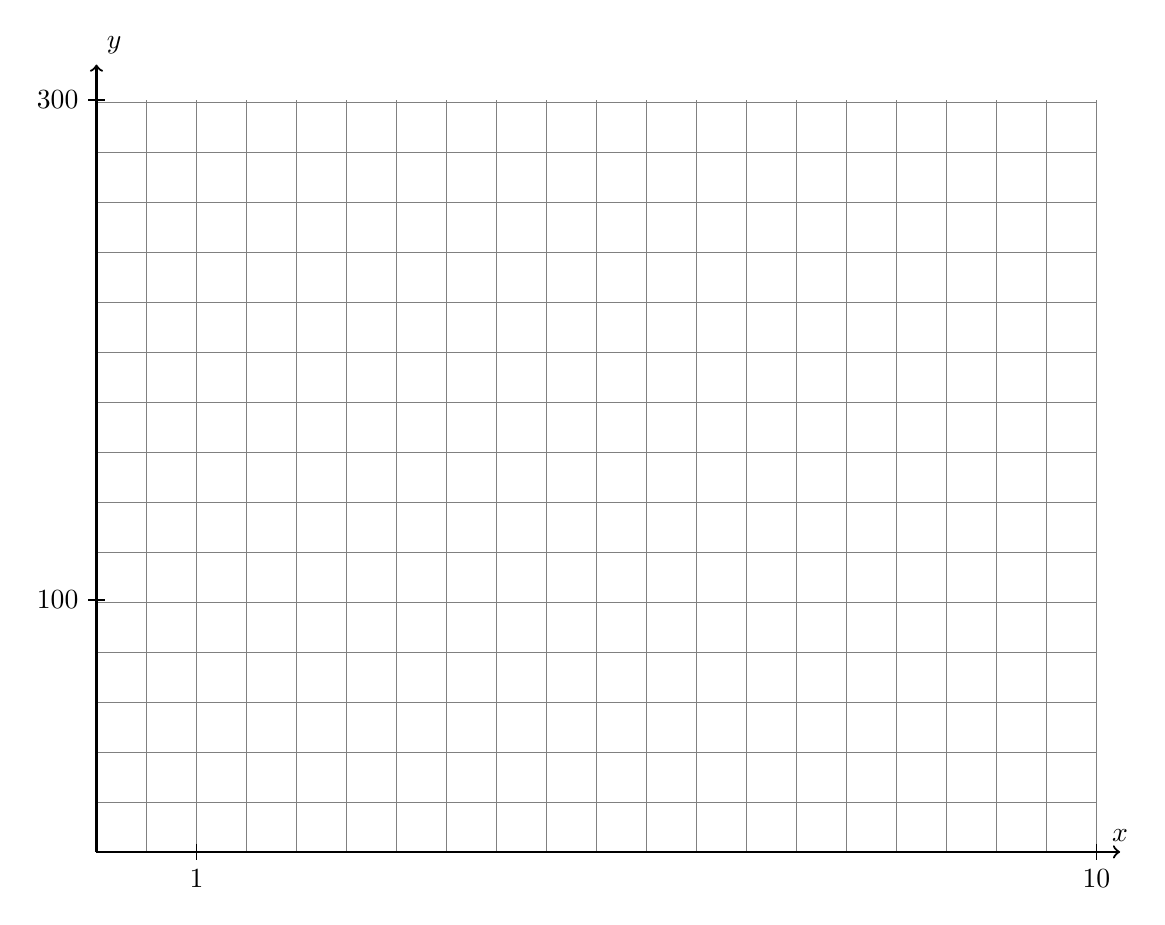
\begin{tikzpicture}
        \draw[step=0.25in,gray,very thin] (0,0) grid (12.7,9.55);
        \draw[thick,->] (0,0) -- (13,0) node[above] {$x$};
        \draw[thick,->] (0,0) -- (0,10) node[above right] {$y$};
        \foreach \x in {1.27} \draw (\x cm,3pt) -- (\x cm,-3pt) node[anchor=north] {$1$};
        \foreach \x in {12.7} \draw (\x cm,3pt) -- (\x cm,-3pt) node[anchor=north] {10};
        \foreach \y in {3.2} \draw (3pt,\y cm) -- (-3pt,\y cm) node[anchor=east] {100};
        \foreach \y in {9.55} \draw (3pt,\y cm) -- (-3pt,\y cm) node[anchor=east] {300};
        \end{tikzpicture}
    \end{center} %Alg2 Regents Jun2017

\item Researchers in a local area found that the population of rabbits with an initial population of 20 grew continuously at the rate of 5\% per month. The fox population had an initial value of 30 and grew continuously at the rate of 3\% per month.\\*[5pt]
Find, to the \emph{nearest tenth of a month}, how long it takes for these populations to be equal. %Alg2 Regents Jan2018

\newpage
\item In New York State, the minimum wage has grown exponentially. In 1966, the minimum wage was \$1.25 an hour and in 2015, it was \$8.75. Algebraically determine the rate of growth to the \emph{nearest percent}.

\item Jim is looking to buy a vacation home for \$172,600 near his favorite southern beach. The formula to compute a mortgage payment, $M$, is $\displaystyle M=P \cdot \frac{r(1+r)^N}{(1+r)^N-1}$ where $P$ is the principal amount of the loan, $r$ is the monthly interest rate, and $N$ is the number of monthly payments. Jim’s bank offers a monthly interest rate of 0.305\% for a 15-year mortgage.\\*[5pt]
With no down payment, determine Jim’s mortgage payment, rounded to the nearest dollar.\\*[3.5in]
Algebraically determine and state the down payment, rounded to the \emph{nearest dollar}, that Jim needs to make in order for his mortgage payment to be \$1100.
 %Alg2 Regents Jun2017 multiple choice

\newpage
\item The value of a certain small passenger car based on its use in years is modeled by $V(t) =28482.698(0.684)^t$, where $V(t)$ is the value in dollars and $t$ is the time in years. Zach had to take out a loan to purchase the small passenger car. The function $Z(t)=22151.327(0.778)^t$, where $Z(t)$ is measured in dollars, and $t$ is the time in years, models the unpaid amount of Zach’s loan over time.\\*[10pt]
Graph $V(t)$ and $Z(t)$ over the interval $0 \leq t \leq 5$, on the set of axes below.
\begin{center}
    
\begin{tikzpicture}
    \draw[step=0.25in,gray,very thin] (0,0) grid (12.7,12.7);
    \draw[thick,->] (0,0) -- (13,0);% node[anchor=north west] {x};
    \draw[thick,->] (0,0) -- (0,13);% node[anchor=south east] {y};
    \end{tikzpicture}
\end{center}
State when $V(t)=Z(t)$, to the \emph{nearest hundredth}, and interpret its meaning in the context of the problem.\\*[10pt]
 %Alg2 Regents Aug2017

\newpage
\item The expression $\displaystyle \left( \frac{m^2}{m^\frac{1}{3}}\right)^{-\frac{1}{2}}$ is equivalent to
\begin{enumerate}
    \item $-\sqrt[6]{m^5}$
    \item $\displaystyle \frac{1}{\sqrt[6]{m^5}}$
    \item $-m \sqrt[5]{m}$
    \item $\displaystyle \frac{1}{m \sqrt[5]{m}}$ \\[.5in]
\end{enumerate} %Alg2 Regents Jan2017 multiple choice


\item An equation to represent the value of a car after $t$ months of ownership is\\ $\displaystyle v=32,000(0.81)^{\frac{t}{12}}$. Which statement is \emph{not} correct?
\begin{enumerate}
    \item The car lost approximately 19\% of its value each month.
    \item The car maintained approximately 98\% of its value each month.
    \item The value of the car when it was purchased was \$32,000.
    \item The value of the car 1 year after it was purchased was \$25,920.
\end{enumerate} %Alg2 Regents Aug2016 MC

\item The function below models the average price of gas in a small town since January 1st.
\[G(t)=-0.0049t^4 + 0.0923t^3 - 0.56t^2 +1.166t+3.23 \text{, where } 0 \leq t \leq 10.\]
If $G(t)$ is the average price of gas in dollars and $t$ represents the number of months since January 1st, the absolute maximum $G(t)$ reaches over the given domain is about what value, to the nearest cent? \\[3in] %Alg2 Regents Jan2018

\end{enumerate}
\end{document}
